\section{Backtracking (Podas)}

	La descripción del problema como la forma de pensarlo son las mismas que el ejercicio anterior.

\subsection{Resolución}
	
	Además de lo dicho en el ejercicio anterior, la idea es podar más el árbol para no recorrer casos donde no nos interese su solución o sea un caso inválido. Para esto tenemos 2 podas, la primera consiste en no considerar conjuntos que no mejoran la respuesta y la segunda consiste en hacer un mejor análisis de la confiabilidad de los agentes. Para la primera consideremos un conjunto con "k" elementos en el, previamente habían "a" agentes mientras que "i" representan los agentes procesados, la poda consiste en que si $k+(a-i)$ <= s, donde s es mi mejor solución hasta el momento, no sigo recorriendo ese rama porque se que no voy a conseguir nada mejor. La otra consiste en hacer un mejor chequeo de la confiabilidad además de lo descripto en el ejercicio anterior, vemos que si el agente a ser agregado confia en otro agente, este último debería formar parte del conjunto por lo que vemos si ya está en el conjunto o si puede ser agregado, para esto vereficamos que no haya nadie que desconfie de este agente, si alguien no confia en él no se agrega al agente al conjunto. 
	
\subsection{Pseudocódigo}  
	
\begin{algorithm}[H]
\caption{BacktrackingPodas}\label{Ej1.1}

\begin{algorithmic}[H]
\Procedure{BacktrackingPodas}{vector(pair(agente, agente)) encuestas, agentes, ConjAgentes}
\If{Si no me quedan agentes para evaluar}
\If{longitud(ConjAgentes) > solucion}
\State solucion $=$ longitud(ConjAgentes)
\EndIf
\State\Return solucion
\EndIf
\If{PuedoAgregarAgente $\wedge$ PuedeSerMejorSolución}
\State Paso Recursivo rama agregueAlAgente
\EndIf
\If{PuedeSerMejorSolución}
\State Paso Recursivo rama NoAgregoAlAgente
\EndIf
\EndProcedure
\end{algorithmic}

\end{algorithm}

\subsection{Complejidad}

	Dado que las podas no agregan complejidad al algoritmo ya que se aprovechan de lo que se hacía antes y en peor caso tengo que recorrer todo el árbol, la complejidad en peor caso sigue siendo lo misma que el ejercicio anterior. O($2^{i}*i^{3}*a^{3}$). 
	
\subsection{Experimentación}

\begin{figure}[h]

\begin{subfigure}{0.5\textwidth}
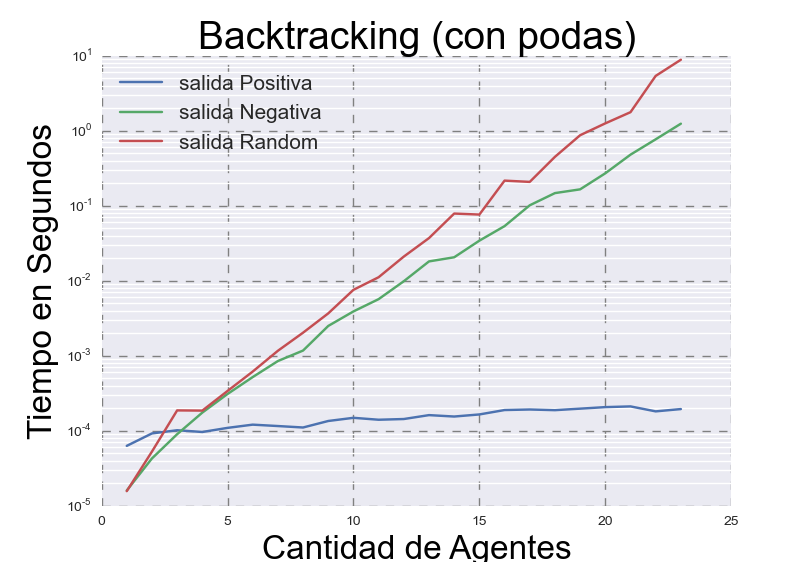
\includegraphics[scale=0.45]{BacktrackingPodasLog.png}
\end{subfigure}
\begin{subfigure}{0.5\textwidth}
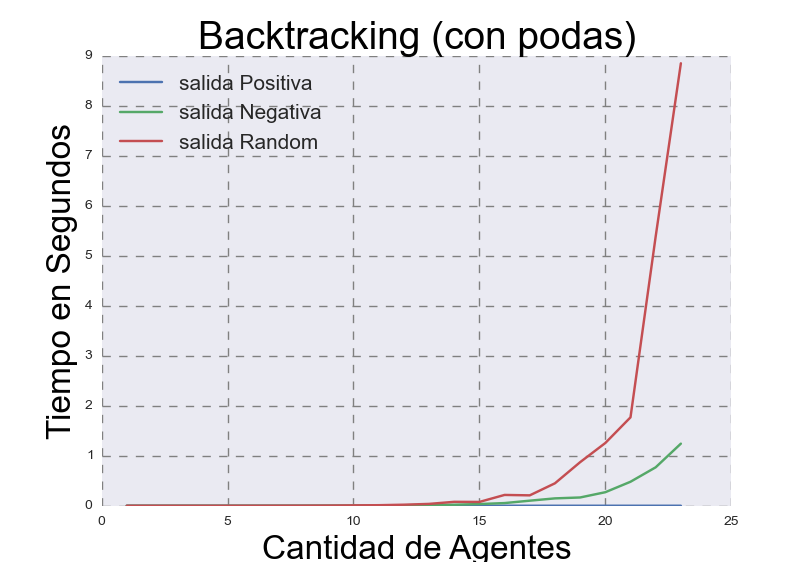
\includegraphics[scale=0.45]{BacktrackingPodas.png}
\end{subfigure}

\end{figure}

	Al igual que en el ejercicio anterior vemos los resultados del algoritmo para diferentes entradas. La muestras fueron calculadas de la misma manera que en el ejercicio anterior.